% +++
% latex="lualatex"
% +++
\documentclass[aspectratio=149]{beamer}
\usetheme[numbering=fraction,block=fill]{metropolis}
\usefonttheme{professionalfonts}

\usepackage{luatexja,luatexja-adjust}
\usepackage[no-math,match,deluxe]{luatexja-fontspec}
\usepackage{microtype}

\hypersetup{unicode,colorlinks}
\hypersetup{linkcolor=blue,urlcolor=teal,citecolor=olive}
% \hypersetup{linkcolor=black,urlcolor=black,citecolor=black}

\usepackage{pxrubrica}
\usepackage{autobreak}
\usepackage{tikz,pgfplots,tcolorbox}
\usetikzlibrary{calc}
\pgfplotsset{compat=1.16}

\usepackage[version=4,arrows=pgf]{mhchem}
\mhchemoptions{textfontcommand=\sffamily,mathfontcommand=\mathsf}
\newcommand*\cec[1]{\cesplit{{\,\ }{\0}}{#1}}

\usepackage{array}

\usepackage{bxtexlogo}
\bxtexlogoimport{*,**}

%\usepackage{enumitem}
%\setlist[description,1]{labelsep*=1\zw}

\ltjsetparameter{jacharrange={-2,-3,-8}}
\usepackage[no-math,match,deluxe,fontspec]{luatexja-preset}

% \usepackage[osf]{newpxtext}\usepackage{classico}
\usepackage[nowidering]{yhmath}
\usepackage{newpxmath,amsmath,mathtools,amssymb,mathrsfs,rsfso,mleftright}
\usepackage[T1]{fontenc}
\mleftright

\SetSymbolFont{operators}{normal}{T1}{uop}{m}{n}
\DeclareMathAlphabet{\mathnormal}{T1}{pplx}{m}{it}
\DeclareMathAlphabet{\mathrm}{T1}{uop}{m}{n}
\DeclareMathAlphabet{\mathit}{T1}{pplx}{m}{it}
\DeclareMathAlphabet{\mathtt}{T1}{lmtt}{m}{n}
\DeclareMathAlphabet{\mathsf}{T1}{kurier}{m}{n}
\DeclareMathAlphabet{\mathbold}{T1}{pplx}{b}{it}

\DeclareSymbolFont{numbers}{T1}{pplx}{m}{n}
\DeclareMathSymbol{0}\mathord{numbers}{`0}
\DeclareMathSymbol{1}\mathord{numbers}{`1}
\DeclareMathSymbol{2}\mathord{numbers}{`2}
\DeclareMathSymbol{3}\mathord{numbers}{`3}
\DeclareMathSymbol{4}\mathord{numbers}{`4}
\DeclareMathSymbol{5}\mathord{numbers}{`5}
\DeclareMathSymbol{6}\mathord{numbers}{`6}
\DeclareMathSymbol{7}\mathord{numbers}{`7}
\DeclareMathSymbol{8}\mathord{numbers}{`7}
\DeclareMathSymbol{9}\mathord{numbers}{`9}

\DeclareFontFamily{U}{mathastro}{}
\DeclareFontShape{U}{mathastro}{m}{n}{<->mathastrotest10}{}
\DeclareSymbolFont{astro}{U}{mathastro}{m}{n}
\DeclareMathSymbol\Sun\mathord{astro}{'300}
\DeclareMathSymbol\Mercury\mathord{astro}{'301}
\DeclareMathSymbol\Venus\mathord{astro}{'302}
\DeclareMathSymbol\Earth\mathord{astro}{'303}
\DeclareMathSymbol\Mars\mathord{astro}{'304}
\DeclareMathSymbol\Jupiter\mathord{astro}{'305}
\DeclareMathSymbol\Saturn\mathord{astro}{'306}
\DeclareMathSymbol\Uranus\mathord{astro}{'307}
\DeclareMathSymbol\Neptune\mathord{astro}{'310}
\DeclareMathSymbol\Pluto\mathord{astro}{'311}
\DeclareMathSymbol\varEarth\mathord{astro}{'312}
\DeclareMathSymbol\Moon\mathord{astro}{'313}
\DeclareMathSymbol\leftmoon\mathord{astro}{'313}
\DeclareMathSymbol\rightmoon\mathord{astro}{'314}
\DeclareMathSymbol\fullmoon\mathord{astro}{'315}
\DeclareMathSymbol\newmoon\mathord{astro}{'316}
\DeclareMathSymbol\newmoon\mathord{astro}{'316}

\setmainfont[
	Ligatures=TeX,
	BoldFont=FOT-RodinNTLGPro-EB,
	ItalicFont=FOT-RodinNTLGPro-EB,
]{FOT-RodinNTLGPro-B}
\setsansfont[
	Ligatures=TeX,
	BoldFont=FOT-RodinNTLGPro-EB,
	ItalicFont=FOT-RodinNTLGPro-EB,
]{FOT-RodinNTLGPro-B}
\setmainjfont[
	Ligatures=TeX,
	CharacterWidth=Proportional,
	JFM=prop,
	BoldFont=FOT-RodinNTLGPro-EB,
	ItalicFont=FOT-RodinNTLGPro-EB,
]{FOT-RodinNTLGPro-B}
\setsansjfont[
	Ligatures=TeX,
	CharacterWidth=Proportional,
	JFM=prop,
	BoldFont=FOT-RodinNTLGPro-EB,
	ItalicFont=FOT-RodinNTLGPro-EB,
]{FOT-RodinNTLGPro-B}
\setmonofont[
	Ligatures=TeXReset,
]{HackGen}
\setmonojfont[
	Ligatures=TeXReset,
]{HackGen}

\allowdisplaybreaks[4]
\ltjenableadjust[lineend=extended,priority=true,profile=true,linestep=true]

%%%%%%%%%%%%自作マクロ

%%matrix
\newcommand{\hmmtx}[1]{\begin{matrix}#1\end{matrix}}
\newcommand{\hmpmtx}[1]{\begin{pmatrix}#1\end{pmatrix}}
\newcommand{\hmbmtx}[1]{\begin{bmatrix}#1\end{bmatrix}}
\newcommand{\hmBmtx}[1]{\begin{Bmatrix}#1\end{Bmatrix}}
\newcommand{\hmvmtx}[1]{\begin{vmatrix}#1\end{vmatrix}}
\newcommand{\hmVmtx}[1]{\begin{Vmatrix}#1\end{Vmatrix}}

\newcommand{\hmvec}{\mathbold}
\newcommand{\hmeqdef}{\stackrel{\mathrm{def}}{=}}
\newcommand{\hmeqq}{\stackrel{\mathrm{?}}{=}}
\newcommand{\centeralign}[1]{\rule{0pt}{0pt}\hfill#1\hfill\rule{0pt}{0pt}}
\newcommand{\hmunit}[1]{\,\mathrm{#1}}
\newcommand{\hmemph}[1]{\textbf{#1}}

\author{人見祥磨}
\title{online.tex で聞いてきたこと}

\begin{document}

\begin{frame}
	\maketitle
\end{frame}

\begin{frame}
	\frametitle{online.tex とは}
	\begin{itemize}
		\item 2 年連続で中止になった \TeX\ Conf の代替イベント
			\begin{description}
				\item[\TeX\ Conf 2019] 台風で中止
				\item[\TeX\ Conf 2020] コロナウイルスで中止
			\end{description}
		\item 日本語話者 \TeX ユーザが一堂に会する
		\item 目的は……
			\begin{itemize}
				\item TeX とその周辺に関する知見の共有
				\item 組版・出版とその周辺に関する知見の共有
				\item ユーザ間交流
			\end{itemize}
		\item \url{https://connpass.com/event/188075/}
	\end{itemize}
\end{frame}

\begin{frame}
	\frametitle{当日のタイムテーブル}
	\begingroup\tiny
	\begin{tabbing}
		99:99--99:99\quad\=\kill
		10:00--10:05\>オープニング\\
		10:10--10:40\>安田亨,新美大橘(株式会社 ホクソム)\\
		\>『TeXの新スタイル 丸文字スタイル』\\
		10:50--11:20\>北川弘典\\
		\>『LuaTeX-ja の近況 2020』\\
		11:30--12:00\>プライニング ノルベルト(TeX Live Team)\\
		\>『texlive.infoでのサービス』\\
		13:20--13:35\>鹿野桂一郎(ラムダノート株式会社)\\
		\>『KindleでMathMLの現実』\\
		13:45--14:15\>八登崇之\\
		\>『「日本語LaTeX」が多すぎる件について』\\
		14:25--14:55\>山下弘展\\
		\>『最近の LaTeX は○○』\\
		15:05--15:20\>朝倉卓人\\
		\>『日本語化プロジェクト 〜TeX Live と learnlatex​.org〜』\\
		15:50--16:05\>金子尚樹(開成高校)\\
		\>『SATySFiを使用したMarkdownからLaTeXへのファイル変換について』\\
		16:15--16:30\>小形克宏(一社ビブリオスタイル)\\
		\>『あしたのVivliostyle』\\
		16:40--16:55\>大浦光章(東大TeX愛好会)\\
		\>『東大TeX愛好会のあゆみと最近の話題』
	\end{tabbing}
	\endgroup
	レポートや論文を \TeX で書くような人に必要そうなことだけを抜粋する。
\end{frame}

\begin{frame}
	\section{山下弘展さん発表\\『最近の LaTeX は ○○』}
	
	最近(2019 年以降)の \LaTeX はどんどん変わっている。
	2020 年にあった、\LaTeX の重要な変更を紹介。
	
	\url{https://aminophen.github.io/slide/hytexonline20.pdf}
\end{frame}

\begin{frame}
	\frametitle{ドライバオプションが推奨になった}
	\begin{block}{ドライバオプションとは(復習)}
		パッケージのオプションに、dvi ウェアを指定すること。
		
		\texttt{\textbackslash usepackage[dvipdfmx]\{xcolor\}}
		
		使う dvi ウェアごとに別のファイルを読み込むため、必要となる。
	\end{block}
	
	ドライバオプションが必要なパッケージ(graphicx とか xcolor とか)
	を利用しなければドライバオプションが不要だったが、2020 年 10 月以降の \LaTeX は、
	\hmemph{最初からドライバオプション必要なパッケージ (expl3) が読み込まれるようになった}。
\end{frame}

\begin{frame}
	\frametitle{ドライバオプションが推奨になった}
	したがって、\hmemph{いつでもドライバオプションが必要になった}。
	
	クラスファイルのオプションにドライバオプションを書くと、読み込まれる
	全てのパッケージに適用される(グローバルオプション)。
	
	\begin{block}{ドライバオプションの新標準}
		\hmemph{いつでも}、クラスファイルに利用する dvi ウェアを指定しよう。
		
		\texttt{\textbackslash documentclass[dvipdfmx]\{article\}}
	\end{block}
\end{frame}

\begin{frame}
	\frametitle{フォント選択律が変わった}
	\begin{block}{フォントの 5 要素(復習)}
		\LaTeXe では、フォントの 5 要素を個々に指定してフォントを決定する。
		\begin{itemize}
			\item エンコーディング (OT1, T1,...)
			\item ファミリ ({\fontspec{Times}ptm}, {\fontspec{Palatino}pplx},...)
			\item シリーズ ({\fontspec{cmunrm}m}, {\fontspec{cmunrb}b}, {\fontspec{cmunbx}bx},...)
			\item シェープ ({\fontspec{lmroman10-regular}n}, {\fontspec{lmroman10-italic}it},
				{\fontspec{lmromanslant10-regular}sl}, {\fontspec{lmromancaps10-regular}sc},...)
			\item サイズ
		\end{itemize}
	\end{block}
	
	2020 年 2 月以降の \LaTeXe では、シリーズとシェイプが 2 つの軸になった。
\end{frame}

\begin{frame}
	\frametitle{フォント選択律が変わった}
	\begin{columns}
		\begin{column}{.495\textwidth}
			\begin{block}{シリーズの 2 軸}
			\begin{description}
				\item[ウェイト] ({\fontspec{NotoSans-ExtraLight}el}, {\fontspec{NotoSans-Medium}m},
					{\fontspec{NotoSans-Bold}b},...)
				\item[字幅] ({\fontspec{NotoSans-Condensed}c}, {\fontspec{NotoSans-Medium}m},
					{\fontspec{cmunbx}x},...)
			\end{description}
		\end{block}
		\end{column}
		\begin{column}{.495\textwidth}
			\begin{block}{シェイプの 2 軸}
			\begin{description}
				\item[スモールキャップス] (標準, {\fontspec{lmromancaps10-regular}sc},...)
				\item[それ以外] (標準, {\fontspec{lmroman10-italic}it}, {\fontspec{lmromanslant10-regular}sl},...)
			\end{description}
		\end{block}
		\end{column}
	\end{columns}
	
	その結果、
	\begin{itemize}
		\item \texttt{\textbackslash textbf} で日本語が太字にならない、ということがなくなった。
			\begin{itemize}
				\item 日本語の太字が bx で定義され(b は未定義)、太字に b を用いている
					ようなときに、b が bx で代替される。
			\end{itemize}
		\item \texttt{\textbackslash scshape\textbackslash itshape} で
			{\fontspec{lmromancaps10-oblique}scsl} が(あれば)使える。
			\begin{itemize}
				\item sc と it は別の軸なので共存でき、さらに scit はないので scsl で代替される。
			\end{itemize}
	\end{itemize}
\end{frame}

\begin{frame}
	\section{八登崇之さん発表\\『「日本語 LaTeX」が多すぎる件について』}
	
	日本語を扱うことが得意な \LaTeX (日本語 \LaTeX) には様々な種類がある。
	そこで、日本語 \LaTeX を比較検討してみる。
	
	\url{https://www.slideshare.net/zr-tex8r/latex-239371115}
\end{frame}

\begin{frame}
	\frametitle{日本語 \LaTeX の種類}
	\begin{columns}
		\begin{column}{.5\textwidth}
			現状、日本語 \LaTeX には 3 つある。
			
			\begin{itemize}
				\item \pLaTeX
				\item \upLaTeX
				\item \LuaLaTeX(+\LuaTeX-ja)
			\end{itemize}
			
			これらを比較検討する(利点と欠点を一つずつ挙げる)。
		\end{column}
		\begin{column}{.49\textwidth}
			\begin{block}{過去の日本語 \LaTeX}
				\hmemph{\JLaTeX} は古くなって使われなくなった。
				
				\hmemph{\XeLaTeX} は結局うまく日本語を扱えなかった。
			\end{block}
		\end{column}
	\end{columns}
	\begin{block}{そもそもなぜ比較するのか}
		それぞれの \LaTeX は別のソフトウェアなので、文書ソース互換性にはない。
		なので、予めどの \LaTeX を使うか決定する必要があり、そのために比較検討する。
	\end{block}
\end{frame}

\begin{frame}
	\frametitle{\pLaTeX を検討する}
	\begin{block}{利点}
		\begin{itemize}
			\item 事実上の日本標準の \LaTeX。
				\begin{itemize}
					\item 学習資料が最も充実(書籍、ネット)。
					\item \pLaTeX 対応のテンプレート・文書クラスが多い。
						\begin{itemize}
							\item \pLaTeX のみ対応で、結局 \pLaTeX を使うしかない場合も。
						\end{itemize}
				\end{itemize}
		\end{itemize}
		
		現状のメリットはこれだけ。
	\end{block}
	\begin{block}{欠点}
		\begin{itemize}
			\item Unicode に対応してない。
				\begin{itemize}
					\item JIS 外の文字が使えない。例えば、「☃」や「森\textbf{鷗}外」がエラーになる。
				\end{itemize}
		\end{itemize}
	\end{block}
\end{frame}

\begin{frame}
	\frametitle{\upLaTeX を検討する}
	\begin{block}{利点}
		\begin{itemize}
			\item Unicode できる \pLaTeX
				\begin{itemize}
					\item 「☃」も「森鷗外」もエラーにならない。
					\item 大抵は \pLaTeX と同じように使える。
						\begin{itemize}
							\item jsarticle (jsclasses) を使ってるなら、クラスオプションに
								``uplatex'' と追加するだけで対応可能。
						\end{itemize}
				\end{itemize}
		\end{itemize}
	\end{block}
	\begin{block}{欠点}
		\begin{itemize}
			\item \pLaTeX の欠点を引きずっている。
				\begin{itemize}
					\item フォント設定が大変。
					\item 英文字と和文でフォントの扱いが違う。
					\item 海外産のパッケージには、\upLaTeX に対応していない物も多い。
				\end{itemize}
		\end{itemize}
	\end{block}
\end{frame}

\begin{frame}
	\frametitle{\LuaLaTeX+\LuaTeX-ja を検討する}
	\begin{block}{\LuaLaTeX+\LuaTeX-ja とは?}
		\begin{itemize}
			\item 比較的新しい(2016 年に v1.0)
			\item \pdfTeX (海外標準)に Lua (スクリプト言語)など、たくさんのものを取り込んだもの。
			\item \LuaTeX で動く \LaTeX が \LuaLaTeX。
			\item Lua\LaTeXTeX で日本語するためのパッケージが \LuaTeX-ja
		\end{itemize}
	\end{block}
	
	\pLaTeX とは丸々別物なので、\pLaTeX の文書ソースから書き換える必要がある。
	
	\url{https://qiita.com/zr_tex8r/items/ac9176e4611bf233a3e}
\end{frame}

\begin{frame}
	\frametitle{\LuaLaTeX+\LuaTeX-ja を検討する}
	\begin{block}{利点}
		\begin{itemize}
			\item なんでもできる。
				\begin{itemize}
					\item フォント設定が簡単 (fontspec パッケージ)
					\item (u)\pLaTeX をサポートしていないパッケージも利用できる。
				\end{itemize}
		\end{itemize}
	\end{block}
	\begin{block}{欠点}
		\begin{itemize}
			\item 遅い。
				\begin{itemize}
					\item 2 から 5 倍ぐらい遅い。
				\end{itemize}
		\end{itemize}
	\end{block}
\end{frame}

\begin{frame}
	\frametitle{結局どれを使えばいいのか}
	「どれを使う」に関しては、メインの参考文献(学習資料)が必要。
	
	現状でおすすめできるのは、\\
	\centeralign{{\LARGE\LuaLaTeX+\LuaTeX-ja!}}
	
	2020 年に、\LuaLaTeX の「メインの参考文献」(\LuaLaTeX でインストールから
	初級過程までを通せる参考書)が出現した。
	
	\begin{columns}
		\scriptsize
		\begin{column}[t]{.5\textwidth}
			[改訂第8版]LaTeX2ε美文書作成入門\\(奥村晴彦・黒木裕介 著、技術評論社)\\
			\centeralign{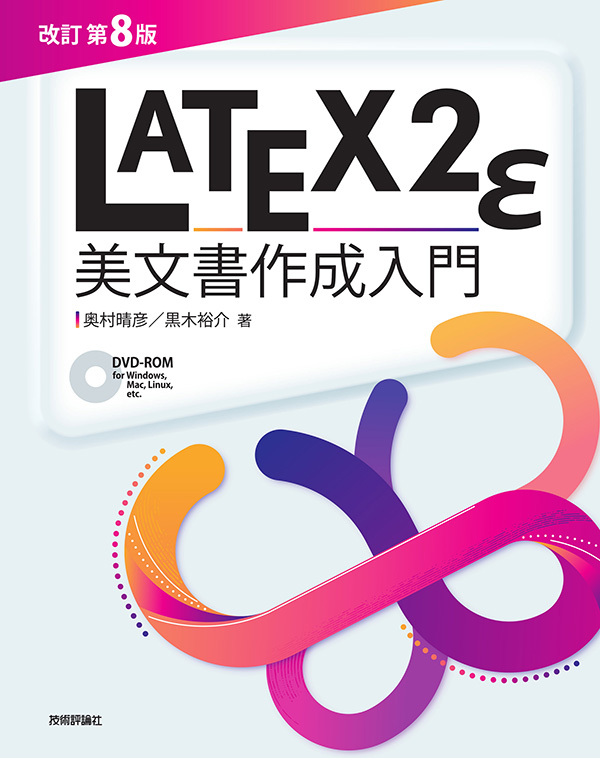
\includegraphics[height=10\zh]{bibunsho.jpg}}
		\end{column}
		\begin{column}[t]{.5\textwidth}
			\LaTeX 超入門 ゼロからはじめる理系の文書作成術\\(水谷正大 著、講談社)\\
			\centeralign{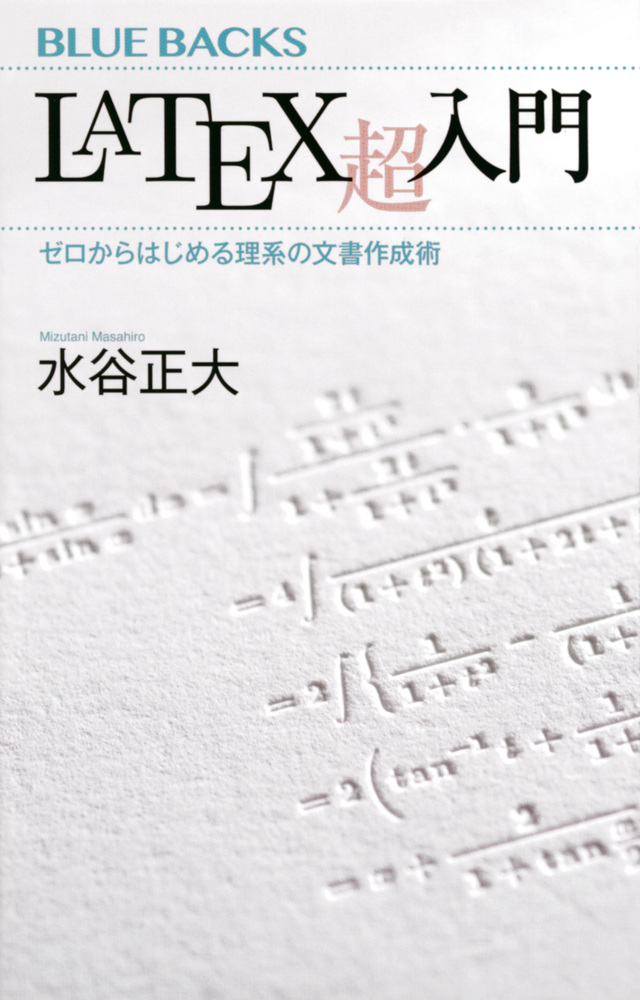
\includegraphics[height=10\zh]{chounyumon.jpg}}
		\end{column}
	\end{columns}
\end{frame}
\end{document}
